% Root file of the TurnAhead paper (ACL Rolling Review submission).
% Build: latexmk -pdf main.tex
\documentclass[11pt]{article}

% Let long URLs in the bibliography break at hyphens.
\PassOptionsToPackage{hyphens}{url}
% "review" for ARR submission; switch to "final" or "preprint" later.
\usepackage[review]{acl}

\usepackage{times}
\usepackage{latexsym}
\usepackage[T1]{fontenc}
\usepackage[utf8]{inputenc}
\usepackage{microtype}
\usepackage{inconsolata}
\usepackage{graphicx}

\usepackage{amsmath}
\usepackage{amssymb}
\usepackage{booktabs}
\usepackage{multirow}
\usepackage{enumitem}
\usepackage{xspace}
\usepackage{xcolor}
\usepackage{algorithm}
\usepackage[noend]{algpseudocode}
% cleveref must come after hyperref, which acl.sty loads.
\usepackage[capitalize,noabbrev]{cleveref}

% !TEX root = main.tex
% ---------------------------------------------------------------------------
% Names. Strategy names are placeholders; change them here only.
% ---------------------------------------------------------------------------
\newcommand{\method}{TurnAhead\xspace}
\newcommand{\stratLaunch}{Anchored Lookahead\xspace}
\newcommand{\stratSandbox}{Sandboxed Execution\xspace}
\newcommand{\stratCommit}{Exact-Input Commit\xspace}
\newcommand{\taubench}{$\tau^2$-bench\xspace}

% ---------------------------------------------------------------------------
% Drafting aids. Remove all uses before submission.
% ---------------------------------------------------------------------------
\newcommand{\planned}[1]{{\color{gray}\itshape [Planned] #1}}

% !TEX root = ../main.tex
% Every number quoted in the paper comes from a file generated by scripts/.
% Generated by scripts/motivation_stats.py. Do not edit by hand.
\newcommand{\MotTasks}{148}
\newcommand{\MotTurns}{762}
\newcommand{\MotToolTurns}{632}
\newcommand{\MotAnchorTurns}{499}
\newcommand{\MotAnchorPct}{79.0}
\newcommand{\MotToolGenPct}{2.3}
\newcommand{\MotReadyPosPct}{8.9}
\newcommand{\MotSlackMedian}{49.3}
\newcommand{\MotSlackSharePct}{91.1}
\newcommand{\MotSlackWallPct}{51.8}
\newcommand{\MotPairs}{487}
\newcommand{\MotNextMedian}{58.6}
\newcommand{\MotSlackOverNext}{0.83}
\newcommand{\MotNextFitsPct}{38.4}
\newcommand{\MotNextHalfPct}{79.1}
\newcommand{\MotNextCoveredPct}{75.4}
\newcommand{\MotInputSame}{481}
\newcommand{\MotInputSamePct}{96.4}
\newcommand{\MotInputText}{6}
\newcommand{\MotInputTag}{12}
\newcommand{\MotInputDiff}{18}
\newcommand{\MotStateCommitted}{26}
\newcommand{\MotStateDiscarded}{10}
\newcommand{\MotStateTotal}{36}
\newcommand{\MotPlotOutside}{8}
\newcommand{\MotCopyMedian}{0.26}
\newcommand{\MotDraftTokenPct}{2.2}
\newcommand{\MotDraftTimePct}{2.2}
\newcommand{\MotDraftForgonePct}{1.0}
\newcommand{\MotStdTasks}{148}
\newcommand{\MotStdTurns}{1500}
\newcommand{\MotStdToolTurns}{1251}
\newcommand{\MotStdAnchorTurns}{958}
\newcommand{\MotStdAnchorPct}{76.6}
\newcommand{\MotStdToolGenPct}{6.7}
\newcommand{\MotStdReadyPosPct}{18.6}
\newcommand{\MotStdSlackMedian}{15.4}
\newcommand{\MotStdSlackSharePct}{81.4}
\newcommand{\MotStdSlackWallPct}{46.6}
\newcommand{\MotStdPairs}{944}
\newcommand{\MotStdNextMedian}{20.6}
\newcommand{\MotStdSlackOverNext}{0.72}
\newcommand{\MotStdNextFitsPct}{33.6}
\newcommand{\MotStdNextHalfPct}{70.1}
\newcommand{\MotStdNextCoveredPct}{69.6}
\newcommand{\MotStdInputSame}{914}
\newcommand{\MotStdInputSamePct}{95.4}
\newcommand{\MotStdInputText}{3}
\newcommand{\MotStdInputTag}{41}
\newcommand{\MotStdInputDiff}{44}
\newcommand{\MotStdStateCommitted}{54}
\newcommand{\MotStdStateDiscarded}{11}
\newcommand{\MotStdStateTotal}{65}
\newcommand{\MotStdPlotOutside}{0}
\newcommand{\MotStdCopyMedian}{0.29}
\newcommand{\MotStdDraftTokenPct}{2.1}
\newcommand{\MotStdDraftTimePct}{2.1}
\newcommand{\MotStdDraftForgonePct}{0.8}

% Generated by scripts/results_stats.py. Do not edit by hand.
\newcommand{\ConStdMs}{39.1}
\newcommand{\ConStdExtraMs}{10.5}
\newcommand{\ConStdTwo}{1.27}
\newcommand{\ConStdThree}{1.39}
\newcommand{\ConStdFour}{1.53}
\newcommand{\ConDetMs}{117.2}
\newcommand{\ConDetExtraMs}{9.3}
\newcommand{\ConDetTwo}{1.08}
\newcommand{\ConDetThree}{1.12}
\newcommand{\ConDetFour}{1.14}
\newcommand{\StdPlanned}{155}
\newcommand{\StdTasks}{141}
\newcommand{\StdGroups}{270}
\newcommand{\StdTurns}{5.3}
\newcommand{\StdMeanNone}{138.8}
\newcommand{\StdMedNone}{128.8}
\newcommand{\StdTailNone}{259.9}
\newcommand{\StdMeanDisp}{134.8}
\newcommand{\StdMedDisp}{121.5}
\newcommand{\StdTailDisp}{268.0}
\newcommand{\StdMeanOurs}{117.7}
\newcommand{\StdMedOurs}{104.2}
\newcommand{\StdTailOurs}{214.7}
\newcommand{\StdSaveOursDisp}{12.7}
\newcommand{\StdSaveOursDispLo}{7.2}
\newcommand{\StdSaveOursDispHi}{17.9}
\newcommand{\StdSpeedOursDisp}{1.15}
\newcommand{\StdTokSaveOursDisp}{11.2}
\newcommand{\StdTokSaveOursDispLo}{9.6}
\newcommand{\StdTokSaveOursDispHi}{12.8}
\newcommand{\StdFasterOursDisp}{97}
\newcommand{\StdMedSaveOursDisp}{14.3}
\newcommand{\StdTailSaveOursDisp}{19.9}
\newcommand{\StdSaveOursNone}{15.2}
\newcommand{\StdSaveOursNoneLo}{10.0}
\newcommand{\StdSaveOursNoneHi}{20.2}
\newcommand{\StdSpeedOursNone}{1.18}
\newcommand{\StdTokSaveOursNone}{15.1}
\newcommand{\StdTokSaveOursNoneLo}{13.3}
\newcommand{\StdTokSaveOursNoneHi}{16.9}
\newcommand{\StdFasterOursNone}{100}
\newcommand{\StdMedSaveOursNone}{19.1}
\newcommand{\StdTailSaveOursNone}{17.4}
\newcommand{\StdSaveDispNone}{2.9}
\newcommand{\StdSaveDispNoneLo}{$-$3.9}
\newcommand{\StdSaveDispNoneHi}{9.3}
\newcommand{\StdSpeedDispNone}{1.03}
\newcommand{\StdTokSaveDispNone}{4.4}
\newcommand{\StdTokSaveDispNoneLo}{3.3}
\newcommand{\StdTokSaveDispNoneHi}{5.5}
\newcommand{\StdFasterDispNone}{80}
\newcommand{\StdMedSaveDispNone}{5.6}
\newcommand{\StdTailSaveDispNone}{$-$3.1}
\newcommand{\StdMatchNone}{52.0}
\newcommand{\StdSolvedNone}{17.4}
\newcommand{\StdMatchDisp}{51.6}
\newcommand{\StdSolvedDisp}{17.8}
\newcommand{\StdMatchOurs}{52.6}
\newcommand{\StdSolvedOurs}{18.5}
\newcommand{\StdMatchDiffOursDisp}{1.0}
\newcommand{\StdMatchDiffOursDispLo}{$-$3.0}
\newcommand{\StdMatchDiffOursDispHi}{5.4}
\newcommand{\StdMatchDiffOursNone}{0.6}
\newcommand{\StdMatchDiffOursNoneLo}{$-$4.1}
\newcommand{\StdMatchDiffOursNoneHi}{5.4}
\newcommand{\StdFailOther}{0}
\newcommand{\StdRunsNone}{310}
\newcommand{\StdFailNone}{18}
\newcommand{\StdFailPctNone}{5.8}
\newcommand{\StdRunsDisp}{310}
\newcommand{\StdFailDisp}{12}
\newcommand{\StdFailPctDisp}{3.9}
\newcommand{\StdRunsOurs}{310}
\newcommand{\StdFailOurs}{18}
\newcommand{\StdFailPctOurs}{5.8}
\newcommand{\StdFailDiffOursDisp}{1.9}
\newcommand{\StdFailDiffOursDispLo}{$-$1.9}
\newcommand{\StdFailDiffOursDispHi}{5.5}
\newcommand{\StdFailDiffOursNone}{0.0}
\newcommand{\StdFailDiffOursNoneLo}{$-$4.5}
\newcommand{\StdFailDiffOursNoneHi}{4.2}
\newcommand{\WinStdWindows}{770}
\newcommand{\WinStdStarted}{754}
\newcommand{\WinStdCommitted}{499}
\newcommand{\WinStdDiscarded}{255}
\newcommand{\WinStdCommitPct}{66.2}
\newcommand{\WinStdRejCall}{132}
\newcommand{\WinStdRejReply}{98}
\newcommand{\WinStdRejInput}{25}
\newcommand{\WinStdRejOther}{0}
\newcommand{\WinStdOverlapMed}{21.8}
\newcommand{\WinStdOverlapCommitPct}{61.2}
\newcommand{\WinStdCommittedPerTask}{1.85}
\newcommand{\OvhStdGenNone}{1.00}
\newcommand{\OvhStdProbePctNone}{0.0}
\newcommand{\OvhStdLostPctNone}{0.0}
\newcommand{\OvhStdGenDisp}{1.03}
\newcommand{\OvhStdProbePctDisp}{3.1}
\newcommand{\OvhStdLostPctDisp}{0.0}
\newcommand{\OvhStdGenOurs}{1.17}
\newcommand{\OvhStdProbePctOurs}{4.6}
\newcommand{\OvhStdLostPctOurs}{12.6}
\newcommand{\SpdStdMsSolo}{36.8}
\newcommand{\SpdStdMsBusy}{44.3}
\newcommand{\SpdStdBusyRatio}{1.20}
\newcommand{\SpdStdTurnTokens}{654}
\newcommand{\SpdStdTurnSeconds}{24.4}
\newcommand{\ReuseStdTurns}{157}
\newcommand{\ReuseStdReplacedPct}{11.4}
\newcommand{\ReuseStdPrefixPct}{4.3}
\newcommand{\ReuseStdSharedPct}{14.0}
\newcommand{\ReuseStdSharedAllPct}{1.6}
\newcommand{\DetPlanned}{155}
\newcommand{\DetTasks}{148}
\newcommand{\DetGroups}{148}
\newcommand{\DetTurns}{5.1}
\newcommand{\DetMeanNone}{375.0}
\newcommand{\DetMedNone}{350.5}
\newcommand{\DetTailNone}{638.7}
\newcommand{\DetMeanDisp}{366.7}
\newcommand{\DetMedDisp}{342.1}
\newcommand{\DetTailDisp}{623.8}
\newcommand{\DetMeanOurs}{293.7}
\newcommand{\DetMedOurs}{267.9}
\newcommand{\DetTailOurs}{522.6}
\newcommand{\DetSaveOursDisp}{19.9}
\newcommand{\DetSaveOursDispLo}{18.1}
\newcommand{\DetSaveOursDispHi}{21.6}
\newcommand{\DetSpeedOursDisp}{1.25}
\newcommand{\DetTokSaveOursDisp}{19.9}
\newcommand{\DetTokSaveOursDispLo}{18.1}
\newcommand{\DetTokSaveOursDispHi}{21.6}
\newcommand{\DetFasterOursDisp}{141}
\newcommand{\DetMedSaveOursDisp}{21.7}
\newcommand{\DetTailSaveOursDisp}{16.2}
\newcommand{\DetSaveOursNone}{21.7}
\newcommand{\DetSaveOursNoneLo}{19.9}
\newcommand{\DetSaveOursNoneHi}{23.5}
\newcommand{\DetSpeedOursNone}{1.28}
\newcommand{\DetTokSaveOursNone}{21.7}
\newcommand{\DetTokSaveOursNoneLo}{19.9}
\newcommand{\DetTokSaveOursNoneHi}{23.5}
\newcommand{\DetFasterOursNone}{140}
\newcommand{\DetMedSaveOursNone}{23.6}
\newcommand{\DetTailSaveOursNone}{18.2}
\newcommand{\DetSaveDispNone}{2.2}
\newcommand{\DetSaveDispNoneLo}{2.0}
\newcommand{\DetSaveDispNoneHi}{2.4}
\newcommand{\DetSpeedDispNone}{1.02}
\newcommand{\DetTokSaveDispNone}{2.2}
\newcommand{\DetTokSaveDispNoneLo}{2.0}
\newcommand{\DetTokSaveDispNoneHi}{2.4}
\newcommand{\DetFasterDispNone}{140}
\newcommand{\DetMedSaveDispNone}{2.4}
\newcommand{\DetTailSaveDispNone}{2.3}
\newcommand{\DetMatchNone}{52.3}
\newcommand{\DetSolvedNone}{16.9}
\newcommand{\DetMatchDisp}{52.3}
\newcommand{\DetSolvedDisp}{16.9}
\newcommand{\DetMatchOurs}{52.3}
\newcommand{\DetSolvedOurs}{16.9}
\newcommand{\DetMatchDiffOursDisp}{0.0}
\newcommand{\DetMatchDiffOursDispLo}{0.0}
\newcommand{\DetMatchDiffOursDispHi}{0.0}
\newcommand{\DetMatchDiffOursNone}{0.0}
\newcommand{\DetMatchDiffOursNoneLo}{0.0}
\newcommand{\DetMatchDiffOursNoneHi}{0.0}
\newcommand{\DetFailOther}{0}
\newcommand{\DetRunsNone}{155}
\newcommand{\DetFailNone}{7}
\newcommand{\DetFailPctNone}{4.5}
\newcommand{\DetRunsDisp}{155}
\newcommand{\DetFailDisp}{7}
\newcommand{\DetFailPctDisp}{4.5}
\newcommand{\DetRunsOurs}{155}
\newcommand{\DetFailOurs}{7}
\newcommand{\DetFailPctOurs}{4.5}
\newcommand{\DetFailDiffOursDisp}{0.0}
\newcommand{\DetFailDiffOursDispLo}{0.0}
\newcommand{\DetFailDiffOursDispHi}{0.0}
\newcommand{\DetFailDiffOursNone}{0.0}
\newcommand{\DetFailDiffOursNoneLo}{0.0}
\newcommand{\DetFailDiffOursNoneHi}{0.0}
\newcommand{\WinDetWindows}{413}
\newcommand{\WinDetStarted}{410}
\newcommand{\WinDetCommitted}{271}
\newcommand{\WinDetDiscarded}{139}
\newcommand{\WinDetCommitPct}{66.1}
\newcommand{\WinDetRejCall}{66}
\newcommand{\WinDetRejReply}{63}
\newcommand{\WinDetRejInput}{10}
\newcommand{\WinDetRejOther}{0}
\newcommand{\WinDetOverlapMed}{60.9}
\newcommand{\WinDetOverlapCommitPct}{58.7}
\newcommand{\WinDetCommittedPerTask}{1.83}
\newcommand{\OvhDetGenNone}{1.00}
\newcommand{\OvhDetProbePctNone}{0.0}
\newcommand{\OvhDetLostPctNone}{0.0}
\newcommand{\OvhDetGenDisp}{1.03}
\newcommand{\OvhDetProbePctDisp}{2.9}
\newcommand{\OvhDetLostPctDisp}{0.0}
\newcommand{\OvhDetGenOurs}{1.18}
\newcommand{\OvhDetProbePctOurs}{4.4}
\newcommand{\OvhDetLostPctOurs}{13.8}
\newcommand{\SpdDetMsSolo}{106.1}
\newcommand{\SpdDetMsBusy}{113.7}
\newcommand{\SpdDetBusyRatio}{1.07}
\newcommand{\SpdDetTurnTokens}{666}
\newcommand{\SpdDetTurnSeconds}{71.0}
\newcommand{\ReuseDetTurns}{76}
\newcommand{\ReuseDetReplacedPct}{10.9}
\newcommand{\ReuseDetPrefixPct}{4.0}
\newcommand{\ReuseDetSharedPct}{11.7}
\newcommand{\ReuseDetSharedAllPct}{1.3}
\newcommand{\DetIdentPlanned}{155}
\newcommand{\DetIdentClean}{148}
\newcommand{\DetIdentSame}{148}
\newcommand{\DetIdentTurns}{762}
\newcommand{\DetIdentFailed}{7}
\newcommand{\DetIdentFailedSame}{7}
\newcommand{\DetIdentMixed}{0}
\newcommand{\AblIdentPlanned}{46}
\newcommand{\AblIdentClean}{43}
\newcommand{\AblIdentSame}{43}
\newcommand{\AblIdentTurns}{217}
\newcommand{\AblIdentFailed}{3}
\newcommand{\AblIdentFailedSame}{3}
\newcommand{\AblIdentMixed}{0}
\newcommand{\StdSamePairsOursDisp}{282}
\newcommand{\StdSameOursDisp}{0}
\newcommand{\StdSamePairsOursNone}{276}
\newcommand{\StdSameOursNone}{0}
\newcommand{\StdSamePairsDispNone}{284}
\newcommand{\StdSameDispNone}{0}
\newcommand{\StdRepeatPairsNone}{146}
\newcommand{\StdRepeatSameNone}{146}
\newcommand{\StdRepeatPairsDisp}{149}
\newcommand{\StdRepeatSameDisp}{139}
\newcommand{\StdRepeatPairsOurs}{138}
\newcommand{\StdRepeatSameOurs}{1}
\newcommand{\AblTasks}{43}
\newcommand{\AblMeanNone}{340.8}
\newcommand{\AblSaveNone}{$-$2.5}
\newcommand{\AblSaveNoneLo}{$-$2.9}
\newcommand{\AblSaveNoneHi}{$-$2.1}
\newcommand{\AblMeanDisp}{332.5}
\newcommand{\AblMeanOurs}{259.1}
\newcommand{\AblSaveOurs}{22.1}
\newcommand{\AblSaveOursLo}{18.1}
\newcommand{\AblSaveOursHi}{25.7}
\newcommand{\AblMeanDefer}{260.5}
\newcommand{\AblSaveDefer}{21.7}
\newcommand{\AblSaveDeferLo}{17.7}
\newcommand{\AblSaveDeferHi}{25.3}
\newcommand{\AblSlowerDefer}{0.6}
\newcommand{\AblSlowerDeferLo}{0.3}
\newcommand{\AblSlowerDeferHi}{0.8}
\newcommand{\AblMeanNoProbe}{260.2}
\newcommand{\AblSaveNoProbe}{21.7}
\newcommand{\AblSaveNoProbeLo}{17.8}
\newcommand{\AblSaveNoProbeHi}{25.4}
\newcommand{\AblSlowerNoProbe}{0.4}
\newcommand{\AblSlowerNoProbeLo}{0.3}
\newcommand{\AblSlowerNoProbeHi}{0.6}
\newcommand{\AblMeanLate}{334.1}
\newcommand{\AblSaveLate}{$-$0.5}
\newcommand{\AblSaveLateLo}{$-$0.6}
\newcommand{\AblSaveLateHi}{$-$0.4}
\newcommand{\AblSlowerLate}{28.9}
\newcommand{\AblSlowerLateLo}{22.6}
\newcommand{\AblSlowerLateHi}{35.3}
\newcommand{\CostDetPred}{20.8}
\newcommand{\CostDetIdeal}{23.7}
\newcommand{\CostDetContention}{2.9}
\newcommand{\CostDetMeasured}{19.9}
\newcommand{\CostDetCorr}{0.998}
\newcommand{\CostDetErrMed}{2.6}
\newcommand{\CostDetBreakeven}{7.9}
\newcommand{\CostStdPred}{11.8}
\newcommand{\CostStdIdeal}{20.6}
\newcommand{\CostStdContention}{8.8}
\newcommand{\CostStdMeasured}{12.7}
\newcommand{\CostStdCorr}{0.238}
\newcommand{\CostStdErrMed}{21.6}
\newcommand{\CostStdBreakeven}{26.9}
\newcommand{\ToolLowFloor}{2}
\newcommand{\ToolLowIdentical}{215}
\newcommand{\ToolLowComparisons}{215}
\newcommand{\ToolLowDispatch}{2.4}
\newcommand{\ToolLowDispatchLo}{2.1}
\newcommand{\ToolLowDispatchHi}{2.8}
\newcommand{\ToolLowIncrement}{22.1}
\newcommand{\ToolLowIncrementLo}{18.1}
\newcommand{\ToolLowIncrementHi}{25.7}
\newcommand{\ToolLowTotal}{24.0}
\newcommand{\ToolLowTotalLo}{20.0}
\newcommand{\ToolLowTotalHi}{27.7}
\newcommand{\ToolLowDefer}{0.6}
\newcommand{\ToolLowDeferLo}{0.3}
\newcommand{\ToolLowDeferHi}{0.8}
\newcommand{\ToolLowNoProbe}{0.4}
\newcommand{\ToolLowNoProbeLo}{0.3}
\newcommand{\ToolLowNoProbeHi}{0.6}
\newcommand{\ToolMidFloor}{10}
\newcommand{\ToolMidIdentical}{215}
\newcommand{\ToolMidComparisons}{215}
\newcommand{\ToolMidDispatch}{9.5}
\newcommand{\ToolMidDispatchLo}{8.4}
\newcommand{\ToolMidDispatchHi}{10.7}
\newcommand{\ToolMidIncrement}{18.8}
\newcommand{\ToolMidIncrementLo}{15.1}
\newcommand{\ToolMidIncrementHi}{22.3}
\newcommand{\ToolMidTotal}{26.5}
\newcommand{\ToolMidTotalLo}{22.7}
\newcommand{\ToolMidTotalHi}{30.0}
\newcommand{\ToolMidDefer}{1.8}
\newcommand{\ToolMidDeferLo}{1.0}
\newcommand{\ToolMidDeferHi}{2.6}
\newcommand{\ToolMidNoProbe}{3.7}
\newcommand{\ToolMidNoProbeLo}{2.8}
\newcommand{\ToolMidNoProbeHi}{4.8}
\newcommand{\ToolHighFloor}{20}
\newcommand{\ToolHighIdentical}{215}
\newcommand{\ToolHighComparisons}{215}
\newcommand{\ToolHighDispatch}{16.4}
\newcommand{\ToolHighDispatchLo}{14.6}
\newcommand{\ToolHighDispatchHi}{18.4}
\newcommand{\ToolHighIncrement}{14.1}
\newcommand{\ToolHighIncrementLo}{10.7}
\newcommand{\ToolHighIncrementHi}{17.3}
\newcommand{\ToolHighTotal}{28.2}
\newcommand{\ToolHighTotalLo}{24.5}
\newcommand{\ToolHighTotalHi}{31.6}
\newcommand{\ToolHighDefer}{1.9}
\newcommand{\ToolHighDeferLo}{0.8}
\newcommand{\ToolHighDeferHi}{3.2}
\newcommand{\ToolHighNoProbe}{7.2}
\newcommand{\ToolHighNoProbeLo}{5.6}
\newcommand{\ToolHighNoProbeHi}{8.9}



% Title as agreed; revisit only if the positioning changes.
\title{\method: Observation-Anchored Cross-Turn Speculation\\for Low-Latency Reasoning Agents}

\author{Anonymous ACL submission}

\begin{document}
\maketitle

% !TEX root = ../main.tex
\begin{abstract}
Speculative tool dispatch can return a tool's observation while a reasoning agent is still generating the call. The next turn normally waits for that generation to finish.
We observe that, after the dispatched tool has returned, the remaining reasoning time covers \MotNextCoveredPct\% of the next turn on average, and that a correctly dispatched call already determines the input of the next turn in \MotInputSamePct\% of the cases.
We present \method, which starts the next turn of the same model as soon as the observation of the dispatched call is ready, runs its tool calls in a sandbox, and commits it only if its input turns out to be identical, token by token, to the real one.
\method needs no training and no additional model, and it leaves the agent's trajectory unchanged when decoding is deterministic.
On \taubench with Qwen3-32B, it reduces the mean task time by \DetSaveOursDisp\% over speculative tool dispatch under deterministic serving, with token-identical trajectories, and by \StdSaveOursDisp\% under standard serving.
Raising the tool latency floor from \ToolLowFloor{} to \ToolHighFloor\,s reduces the additional saving over dispatch from \ToolLowIncrement\% to \ToolHighIncrement\% on the ablation subset.
\end{abstract}


% !TEX root = ../main.tex
\section{Introduction}
\label{sec:intro}

Agents built on large language models solve tasks in turns: the model reads the conversation so far, emits a tool call, and continues from the tool's observation~\citep{yao2023react}.
With a reasoning model, every turn first thinks through the situation, often for hundreds of tokens, before it emits its call.
A single customer-service task then takes minutes, and almost all of this time is the model's own generation, one turn after another.

Recent work removes the part of this time that is spent waiting for tools.
Speculative tool dispatch predicts the call while the model is still reasoning and executes it at once, so that the observation is ready when the model asks for it~\citep{nichols2025speculative,sui2026paste,bai2026spork}.
In its self-speculative form, the prediction comes from the target model itself and needs no training~\citep{bai2026spork}.
But this hides only the tool latency.
When a tool answers within seconds and a turn reasons for much longer, little is gained: with the \ToolLowFloor\,s tool latency of prior evaluations~\citep{bai2026spork}, speculative tool dispatch saves \DetSaveDispNone\% of the end-to-end time in our experiments.
The next turn still starts only when the current turn has finished.
A second line of work does start future steps early, but it takes them from a separate proposer, a cheaper agent or a trained drafter, that must guess what the target model will decide~\citep{hua2024isp,guan2025dsp,ye2026speculative,xu2026leap}.
Its gain depends on how often the proposer agrees with the target, and a trained proposer has to be fitted to each workload.

We start from the time that remains once the tool is off the critical path.
With speculative tool dispatch, a correct call is dispatched in \MotAnchorPct\% of the tool-calling turns, and its observation is ready after a median of \MotReadyPosPct\% of the turn's generation time.
The model then keeps reasoning until it writes the same call, a pattern that has also been reported by \citet{anon2026eta}.
We call this remaining time the \emph{slack} and find two properties of it (\cref{sec:motivation}).
First, the slack is long enough to cover much of the following turn. The median ratio of slack to next-turn duration is \MotSlackOverNext, and on average \MotNextCoveredPct\% of the next turn would fit into it.
Second, the input of the next turn is already determined.
The history keeps only the final output of a turn and not its reasoning, so the next input consists of the conversation so far, the call, and its observation.
Built from the dispatched call, it is identical to the real next input, token by token, in \MotInputSamePct\% of these turns.
During the slack, the agent thus waits for the model to confirm a call that has already been executed, while everything the next turn needs is at hand.

We present \method, which uses the slack to run the next turn (\cref{fig:overview}).
As soon as the observation of the dispatched call is ready, \method starts the next turn on the same target model, from the input that would follow if the current turn ended with exactly this call.
When the current turn finishes, \method keeps the early turn only if its input is identical to the real next input.
Otherwise it discards the early turn and runs the next turn as usual.
Three strategies make this safe.
\stratLaunch starts the next turn at the observation of the dispatched call, so that it builds on a real tool result and not on a predicted one.
\stratSandbox runs the tool calls of unconfirmed turns on copies of the environment, so that a discarded turn leaves no trace.
\stratCommit accepts the early turn only if its whole input matches token by token.
When decoding is deterministic, a committed turn is then exactly the turn that serial execution would have produced.
\method needs no training and no second model, because the early turn is the target model's own turn.

We evaluate \method on the airline and retail domains of \taubench with Qwen3-32B.
Under deterministic serving, it reduces the mean task time by \DetSaveOursDisp\% compared with speculative tool dispatch (\DetSpeedOursDisp$\times$) and by \DetSaveOursNone\% compared with the serial loop, and all configurations produce the same trajectory, token for token, on every task.
Under standard serving, the saving over speculative tool dispatch is \StdSaveOursDisp\%, with comparable gold-action match rates.
A cost model with a single measured parameter, the slowdown of two concurrent requests, predicts both savings from runs without \method (\CostDetPred\% and \CostStdPred\%).
It also states when the method pays off: the share of overlap time spent on committed successors must exceed the relative cost of the second request.
Longer tool latencies leave less slack for the successor. On the same ablation tasks, its incremental saving falls to \ToolHighIncrement\% at a \ToolHighFloor\,s tool floor.

Our contributions are as follows.
\begin{itemize}[leftmargin=*,itemsep=2pt,topsep=3pt]
\item We show that an agent with speculative tool dispatch spends about half of its end-to-end time (\MotSlackWallPct\%) in slack, that the slack can hold most of the next turn, and that a correctly dispatched call and its observation determine the input of the next turn in \MotInputSamePct\% of the cases.
\item We propose \method, a training-free method that runs the next turn of the target model inside the slack, with sandboxed tool execution and an exact-input commit rule that leaves the trajectory unchanged under deterministic decoding.
\item We show that \method reduces the task time by \DetSaveOursDisp\% over speculative tool dispatch with identical trajectories, and we give a cost model that explains its savings under two serving modes.
\end{itemize}

% Draft rendering from scripts/fig_overview.py; to be replaced by the hand-drawn vector figure.
\begin{figure*}[t]
\centering
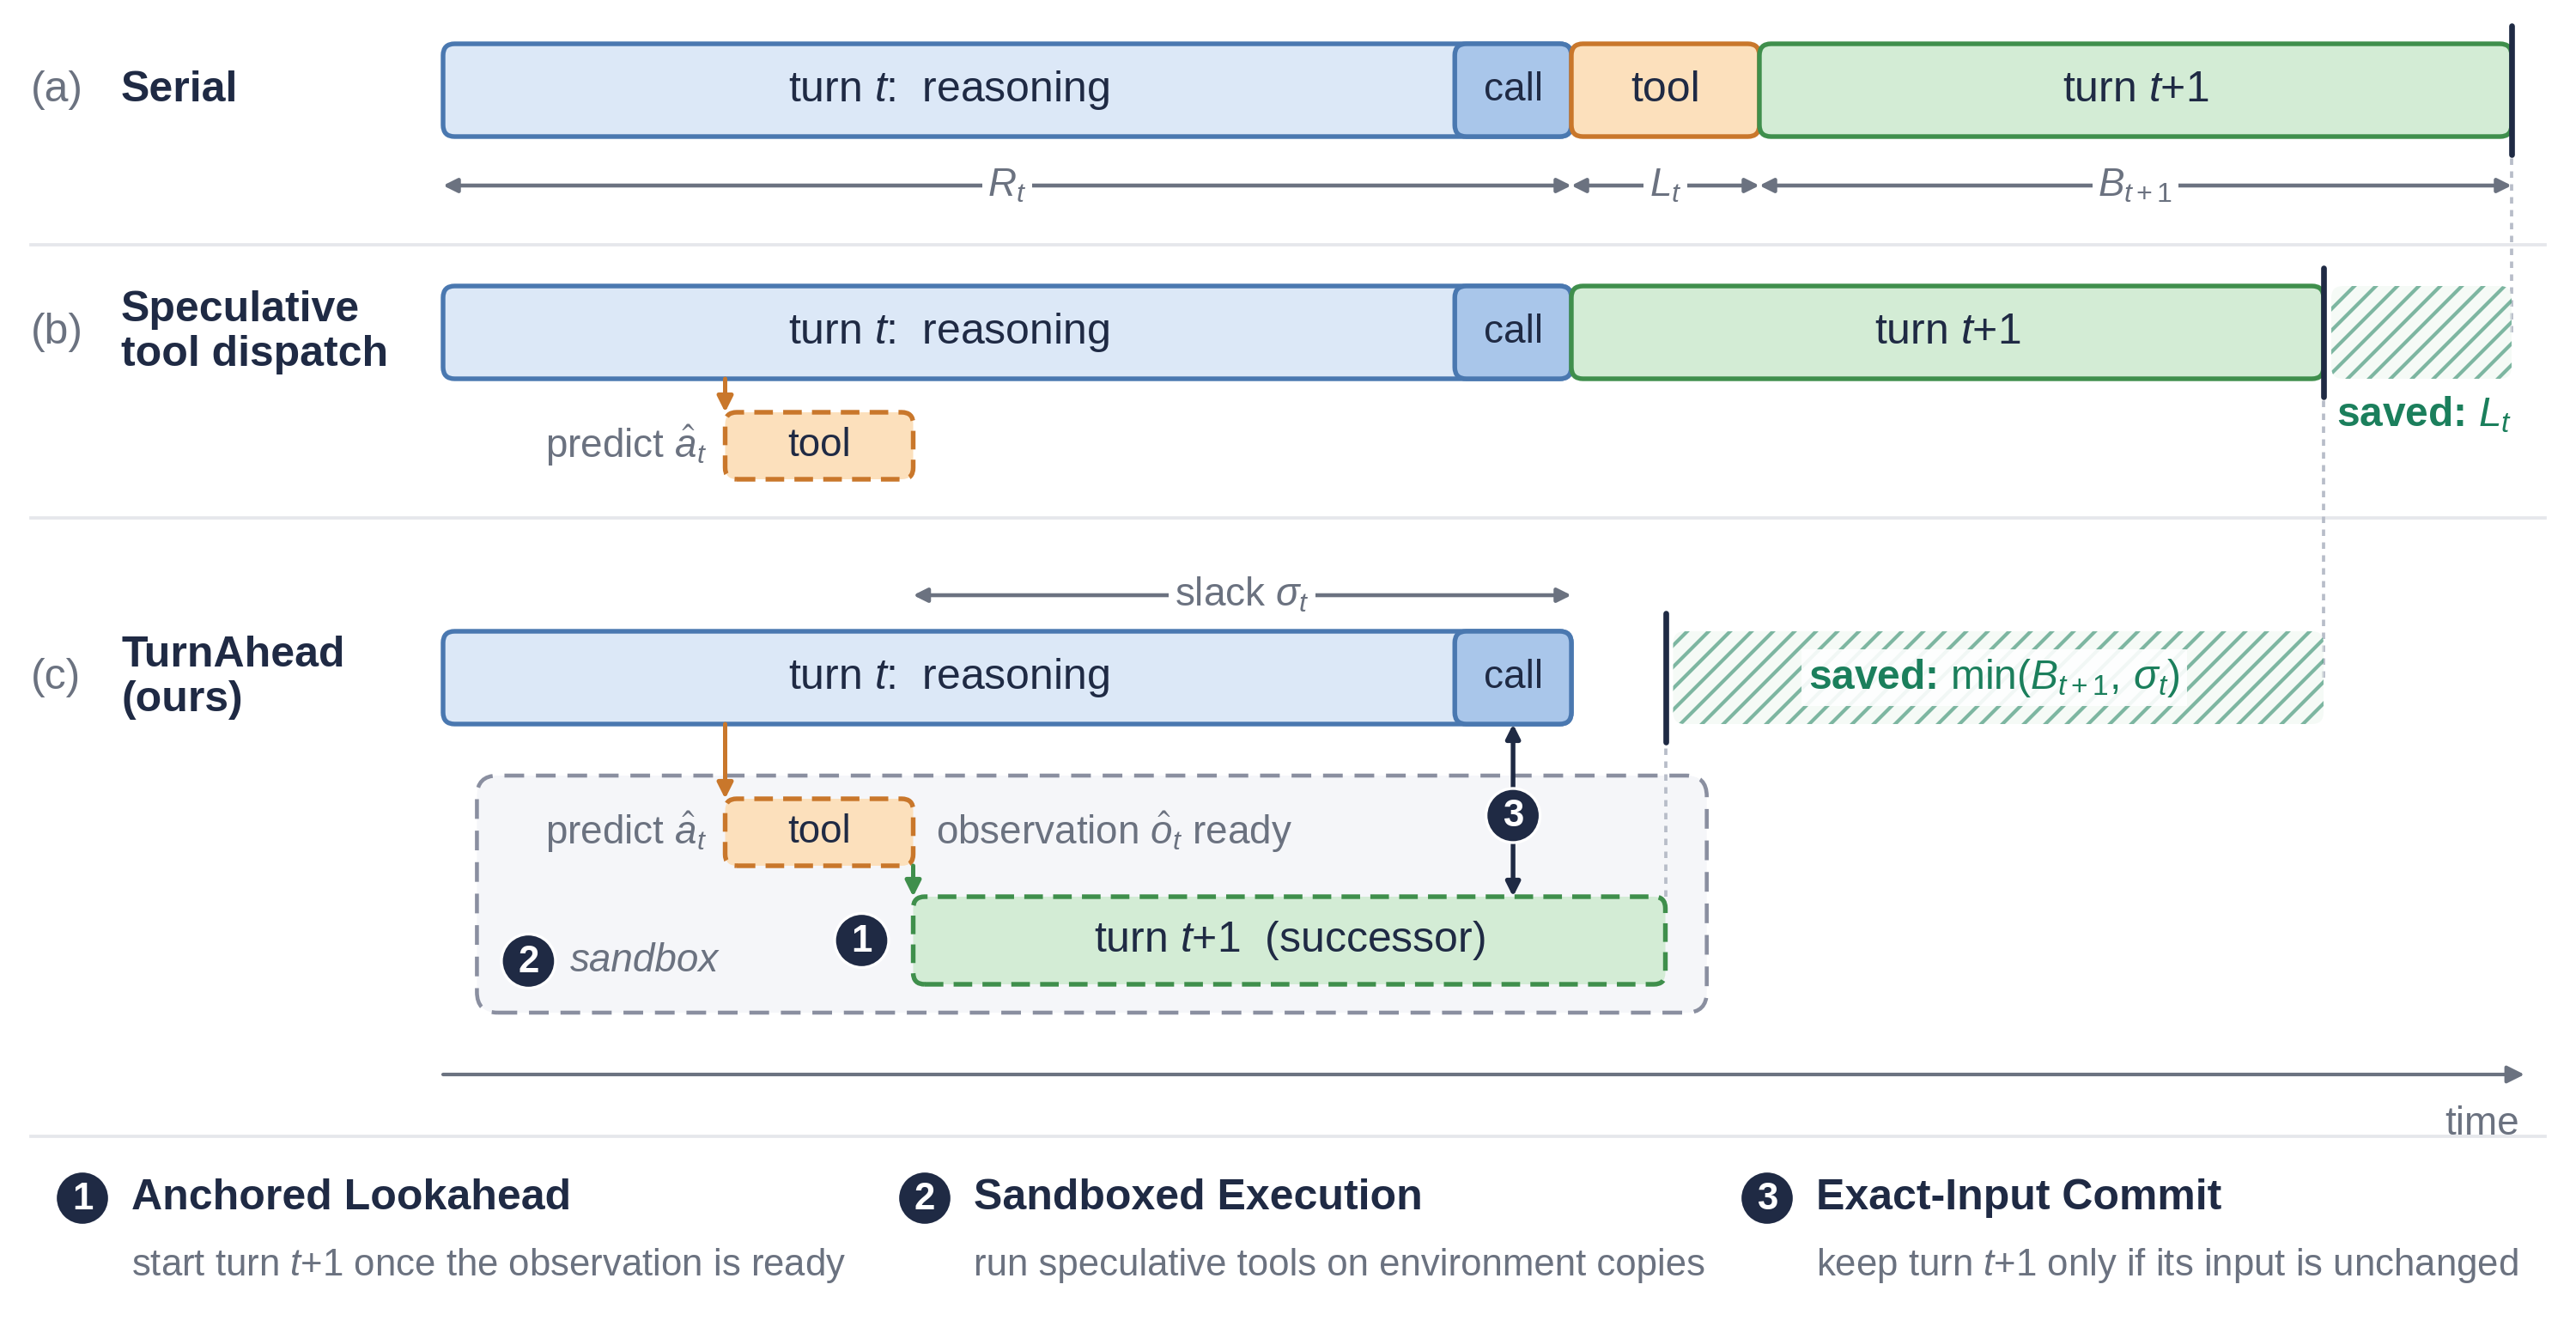
\includegraphics[width=\textwidth]{figures/fig1_overview.png}
\caption{One window of two turns. (a) Serial execution. (b) Speculative tool dispatch predicts the call during reasoning and hides the tool latency $L_t$. (c) \method also starts turn $t{+}1$ once the observation is ready, runs it in a sandbox, and keeps it only if its input is unchanged when turn $t$ ends. Durations are illustrative.}
\label{fig:overview}
\end{figure*}

% !TEX root = ../main.tex
\section{Background and Related Work}
\label{sec:background}

\paragraph{Reasoning agents and speculative tool dispatch.}
A tool-using agent works in turns~\citep{yao2023react}.
In each turn the model reads the conversation so far, reasons, and emits a tool call.
The tool returns an observation, which is appended to the conversation and starts the next turn.
With a reasoning model, one turn can decode hundreds of tokens before the call appears.
The loop is serial: the tool cannot start before the call is written, and the next turn cannot start before the observation exists.

One line of work takes the tool off this critical path by predicting the call and executing it while the model is still generating~\citep{nichols2025speculative,sui2026paste,huang2025spagent,li2026specmemory,bai2026spork}.
In its self-speculative form, no extra model is needed~\citep{bai2026spork}.
A probe request continues the model's own reasoning prefix and is forced to write a tool call.
If the probe is confident, the call is executed at once.
The result is used only if the model later emits the same call, and the probe's tokens can serve as drafts when the model writes it.
We build on this mechanism and call it \emph{speculative tool dispatch}.
Its benefit is bounded by the tool latency, which is small when tools are fast and reasoning is long.

\paragraph{Cross-turn action speculation.}
A second line of work starts future steps before the current one is confirmed.
Interactive and Dynamic Speculative Planning let a cheaper approximation agent run ahead of the target agent, which verifies each step~\citep{hua2024isp,guan2025dsp}.
Speculative Actions formulates this propose--verify pattern for general agent actions and analyzes when it is lossless~\citep{ye2026speculative}.
LEAP trains a small drafter on the target's own actions, executes the drafted actions in a copy of the environment, and lets the target verify the resulting contexts concurrently~\citep{xu2026leap}.
Other systems speculate multi-call macros~\citep{liu2026smc}, combine fast and slow reasoning modes~\citep{zhong2026dualspec}, or predict the observation instead of waiting for the tool~\citep{chen2026aospec,montgomery2026obsspec}.

These methods obtain the future input from a separate component: a cheaper or trained proposer for the action, or a learned model for the observation.
Their gain depends on how often this component agrees with the target, and a trained proposer must be fitted to each workload.
\method needs no such component.
It takes the action from the target's own unfinished turn and the observation from actually executing that action.
It also commits a turn only when its entire input is unchanged, which targets identity of whole trajectories rather than of single actions (\cref{sec:method:commit}).

\paragraph{Faster reasoning.}
Speculative decoding accelerates generation inside a turn at the token level and preserves the model's output~\citep{leviathan2023fast,chen2023accelerating}.
It is orthogonal to \method.
ETA observes, as we do in \cref{sec:motivation}, that reasoning continues long after the dispatched tool has returned, and it ends the reasoning early once the observation arrives~\citep{anon2026eta}.
This shortens the turn but changes what the model generates.
\method keeps the reasoning intact and uses the remaining time to run the next turn.

% !TEX root = ../main.tex
\section{Motivation}
\label{sec:motivation}

We examine where a reasoning agent spends its time once speculative tool dispatch is in place.
The analysis uses the runs of speculative tool dispatch from \cref{sec:experiments} under deterministic serving: Qwen3-32B on the airline and retail domains of \taubench, with \MotTasks{} tasks, \MotTurns{} turns, and a \ToolLowFloor\,s floor on tool latency.
\Cref{app:results} repeats it for standard serving, where turns are shorter and the picture is the same.

\subsection{The Slack Can Hold the Next Turn}
\label{sec:motivation:slack}

Speculative tool dispatch settles the tool call early.
In \MotAnchorTurns{} of the \MotToolTurns{} tool-calling turns (\MotAnchorPct\%), a call is dispatched during reasoning and equals the call that the model finally emits.
In these turns the observation is ready after a median of \MotReadyPosPct\% of the turn's generation time.
The model then keeps reasoning.
We call the time from the moment the observation is ready to the end of the turn's generation the \emph{slack}.
Its median is \MotSlackMedian\,s, which is \MotSlackSharePct\% of the turn's generation time, and the slack of all these turns adds up to \MotSlackWallPct\% of the end-to-end time.
Tool execution, in contrast, amounts to only \MotToolGenPct\% of the generation time.
ETA reports the same pattern in a similar setting~\citep{anon2026eta}.
Reusing the probe's tokens as drafts when the model writes its call is bounded in the same way: the accepted draft tokens are \MotDraftTokenPct\% of all generated tokens.

We ask a further question about the slack: is it long enough to do the work of the next turn?
\Cref{fig:slack} compares each slack with the duration of the turn that follows.
The median next turn takes \MotNextMedian\,s, and the median ratio of slack to next-turn duration is \MotSlackOverNext.
In \MotNextFitsPct\% of the \MotPairs{} pairs the whole next turn would fit into the slack, and in \MotNextHalfPct\% at least half of it would.
On average, \MotNextCoveredPct\% of the next turn could run inside the slack.

\begin{figure}[t]
\centering
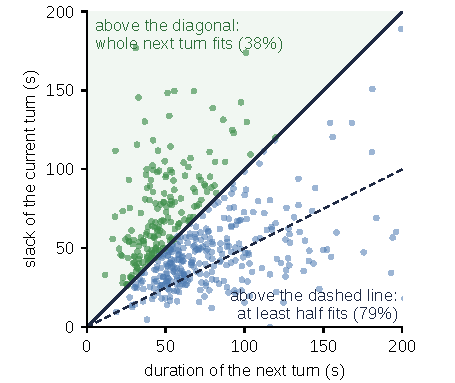
\includegraphics[width=\columnwidth]{figures/fig2_slack.pdf}
\caption{Slack of a turn against the duration of the turn that follows, for the \MotPairs{} pairs of consecutive turns in which the dispatched call was correct (Qwen3-32B, \taubench). \MotPlotOutside{} pairs beyond 200\,s are not shown.}
\label{fig:slack}
\end{figure}

\subsection{The Next Input Is Already Determined}
\label{sec:motivation:input}

Running the next turn early requires its input.
That input is the conversation so far plus what the current turn adds to it.
The turn's reasoning is not part of what is added.
The model developers recommend that the history keep only the final output of each turn, without its thinking content~\citep{qwen2025qwen3card,qwen2026qwen35card}, and agent harnesses follow this practice~\citep{bai2026spork,xu2026leap}.\footnote{The reference chat templates of both models re-insert reasoning that the caller supplies for assistant turns after the last user message. Our harness never supplies it, for any method.}
A tool-calling turn therefore adds only its visible output, which is normally the call alone, and the observation.
Both are available during the slack: the call has been predicted, and the observation has been obtained by executing it.

We test this on the same \MotAnchorTurns{} turns.
For each turn, we build the next input from the dispatched call and its observation alone and compare it with the input that the agent actually used.
The two are identical, token by token, in \MotInputSame{} cases (\MotInputSamePct\%).
In the other \MotInputDiff{}, the model's output contained more than the call: visible text before the call (\MotInputText{} cases) or a malformed closing tag that stayed in the history (\MotInputTag{} cases).

\subsection{Challenges}
\label{sec:motivation:challenges}

The two observations suggest starting the next turn inside the slack.
Doing so without changing the agent's behavior raises three challenges.

\paragraph{When to start, and from which input.}
The current turn has not finished when the next one should start, so its final call is unknown.
A correct call has been dispatched in \MotAnchorPct\% of the tool-calling turns, but not in the rest.
The next turn must start from an input that is available early and is likely to be the real one.

\paragraph{Side effects.}
A turn that starts early calls tools of its own before anyone knows whether it will be kept.
Some of these calls change state.
In the \method runs of \cref{sec:experiments}, \MotStateTotal{} early turns changed the database, for example through returns or flight changes, and discarded turns account for \MotStateDiscarded{} of them.
Such calls must not reach the real environment before the turn is confirmed.

\paragraph{When to keep the result.}
A matching call does not guarantee a matching input (\cref{sec:motivation:input}).
A turn that ran on a different input is not the turn the serial agent would have produced, and keeping it would change the trajectory.

\Cref{sec:method} addresses these challenges with \stratLaunch, \stratSandbox, and \stratCommit, respectively.

% !TEX root = ../main.tex
\section{\method}
\label{sec:method}

\subsection{Overview}
\label{sec:method:overview}

\method runs the next turn while the current turn is still reasoning (\cref{fig:overview}).
Consider two consecutive turns $t$ and $t{+}1$ of the target model.
We call turn $t$ the \emph{parent}.
While the parent reasons, speculative tool dispatch predicts its call, $\hat a_t$, and executes it, which yields an observation $\hat o_t$.
As soon as $\hat o_t$ is ready, \method starts turn $t{+}1$ on the same model, from the input that would follow if the parent ended with exactly this call.
We call this early run the \emph{successor}.
When the parent finishes, \method checks whether the successor ran on the right input.
If so, the successor is committed as turn $t{+}1$, including the work it has already done.
If not, it is discarded and turn $t{+}1$ runs as usual.

Three strategies make this work.
\stratLaunch decides when the successor starts and how its input is built (\cref{sec:method:launch}).
\stratSandbox keeps the tool calls of unconfirmed turns away from the real environment (\cref{sec:method:sandbox}).
\stratCommit decides whether the successor may be kept (\cref{sec:method:commit}).
\Cref{alg:window} summarizes one window.

\begin{algorithm}[t]
\caption{One \method window. \textsc{Turn} runs one turn of the target model; \textsc{Check} is the test of \cref{sec:method:commit}.}
\label{alg:window}
\small
\begin{algorithmic}[1]
\Require input $X_t$, history $H_t$, environment $S_t$
\State $P \gets \textsc{Turn}(X_t, S_t)$;\; $C \gets \varnothing$
\State $(\hat a,\hat o,\hat S) \gets \textsc{Dispatch}(P)$ \Comment{on a copy of $S_t$}
\If{$\textsc{Reasoning}(P)$} \Comment{\S\ref{sec:method:launch}}
  \State $\hat X \gets \textsc{Render}(H_t\oplus\langle\hat a,\hat o\rangle)$
  \State $C \gets \textsc{Turn}(\hat X, \textsc{Copy}(\hat S))$ \Comment{\S\ref{sec:method:sandbox}}
\EndIf
\State $(X_{t+1}, S_{t+1}) \gets \textsc{Await}(P)$
\If{$C\neq\varnothing$ \textbf{and} $\textsc{Check}(C, P)$} \Comment{\S\ref{sec:method:commit}}
  \State $\textsc{Adopt}(\textsc{Await}(C))$
\Else
  \State $\textsc{Cancel}(C)$;\; $\textsc{Turn}(X_{t+1}, S_{t+1})$
\EndIf
\end{algorithmic}
\end{algorithm}

\paragraph{Time saved.}
Let $R_t$ be the generation time of the parent, $\tau_t$ the time at which $\hat o_t$ is ready, and $B_{t+1}$ the duration of turn $t{+}1$.
With speculative tool dispatch alone, the two turns take $R_t+B_{t+1}$.
With a committed successor they take $\max(R_t,\,\tau_t+B_{t+1})$, which saves
\begin{equation}
  \Delta T_t=\min\big(B_{t+1},\,\sigma_t\big),
  \qquad \sigma_t=R_t-\tau_t,
  \label{eq:saving}
\end{equation}
where $\sigma_t$ is the slack of \cref{sec:motivation:slack}.
The saving is limited by the slack and by the length of the next turn, not by the tool latency, so it adds to what speculative tool dispatch already saves.

The successor shares the server with the parent.
Suppose that each of two concurrent requests runs $s\ge 1$ times slower than it would alone.
A committed window then saves $(2-s)\,\Delta T_t$, and a discarded successor delays its parent by $(s-1)$ times the time for which the two overlap (\cref{app:consistency}).
If committed windows account for a fraction $p$ of the total overlap, a window saves about $(p-(s-1))$ times its overlap on average.
\method therefore pays off when this overlap-weighted commit rate exceeds the relative cost of the second request, and \cref{sec:exp:analysis} measures both.

\paragraph{Losslessness.}
We call an acceleration \emph{lossless} if the committed trajectory is the same as under serial execution: every visible output, tool call, and observation, and the final environment state.
\method is designed to be lossless when decoding is deterministic (\cref{sec:method:commit}).

\subsection{\stratLaunch}
\label{sec:method:launch}

\paragraph{When to start.}
The successor starts at the moment the observation of the dispatched call arrives, provided that the parent is still reasoning, that is, it has neither closed its reasoning nor begun to write its call.
We refer to the dispatched call together with its observation as the \emph{anchor} of the window.
Starting at the anchor gives the successor the whole slack.
If the parent is already writing its call, the slack is almost over and \method does not start a successor.

\paragraph{Which input to use.}
The successor's input is rendered from the committed history $H_t$ extended by the anchor:
\begin{equation}
  \hat X_{t+1}=\mathrm{Render}\big(H_t\oplus\langle\hat a_t,\hat o_t\rangle\big).
  \label{eq:input}
\end{equation}
The assistant message consists of the call $\hat a_t$ alone, and the tool message of $\hat o_t$.
Following \cref{sec:motivation:input}, the parent's reasoning is left out, as it would be in the real history, and no other visible text is assumed.

\paragraph{What the successor runs.}
The successor is a complete turn of the target model with the same decoding configuration as any other turn.
It reasons in full and emits its own call.
No smaller model, prompt variant, or training is involved, so its output is what the target itself produces on $\hat X_{t+1}$.
Speculative tool dispatch stays active inside the successor, so the successor's own tool call is overlapped as well.

\paragraph{Windows.}
\method groups turns into disjoint windows $(1,2),(3,4),\dots$
A successor does not start a successor of its own, and the next window starts from the committed history.
A window never extends beyond a reply to the user, because the following input depends on the user's answer.
A depth of one limits the wasted work to at most one turn per window.

\paragraph{Other anchor sources.}
\stratLaunch needs only an anchor: a candidate call and its observation that are available before the parent ends.
We obtain it from speculative tool dispatch, which requires no training.
A trained action drafter~\citep{xu2026leap} or a memory of past trajectories~\citep{li2026specmemory} could supply it instead, and the rest of \method would stay the same.
We do not evaluate such sources.

\subsection{\stratSandbox}
\label{sec:method:sandbox}

Both the dispatched call and the calls of the successor run before the parent has confirmed them.
In \taubench, such calls cancel reservations, issue refunds, and modify orders.
\method therefore executes them on copies of the environment, at two levels.

\paragraph{First level: the dispatched call.}
The call $\hat a_t$ is executed on a copy of the current environment.
Its observation $\hat o_t$ is therefore a real tool result, not a prediction.
If the parent later emits the same call, this copy becomes the committed environment and the tool is not run again.
Otherwise the copy is dropped.

\paragraph{Second level: the successor.}
The successor runs on a second copy, taken from the first one after $\hat a_t$ has been applied.
A separate copy is necessary because the first copy may become the committed environment as soon as the parent ends, while it is still open whether the successor will be kept.
The tool calls of the successor change only the second copy.

\paragraph{Adoption.}
When the successor is committed, its copy replaces the environment.
When it is discarded, the copy is dropped.
Every tool call thus takes effect at most once, and only after the turn that issued it has been validated.

\paragraph{Deferred execution.}
Copying presupposes that the effects of a tool live in state that can be copied.
For tools with external effects, such as sending a message, \method offers a deferred mode.
The successor generates as usual, but its tool calls are held until the commit decision and run only if the successor is kept.
Only the model computation is then speculative, and the saving is smaller (\cref{sec:exp:ablation}).

\subsection{\stratCommit}
\label{sec:method:commit}

When the parent ends, its real output is known.
If it ends with a reply to the user instead of a tool call, the successor is discarded.
Otherwise the parent's call is committed as usual, which fixes the real observation $o_t$, the real environment, and the real next input $X_{t+1}$.

\paragraph{The check.}
The successor is kept only if five conditions hold:
(i) the dispatched call equals the parent's call in tool name and in every argument;
(ii) the two observations have the same hash;
(iii) the environment from which the successor started has the same fingerprint as the committed environment;
(iv) the successor's input $\hat X_{t+1}$ is identical, token by token, to $X_{t+1}$; and
(v) the decoding configuration is the same.
Condition (iv) is the central one.
As \cref{sec:motivation:input} shows, a matching call does not always give a matching input, and a turn generated from a different input is not the turn the serial agent would have produced.
Conditions (i) and (ii) follow from (iv) and serve to report why a successor was rejected.
Conditions (iii) and (v) cover what the input does not show: the environment behind the conversation and the settings of the request.

\paragraph{Commit.}
If the check passes, \method waits for the successor to finish, repeats the check, and adopts the successor's turn together with its environment copy.
The time that the successor spent running inside the parent's slack is the saving of \cref{eq:saving}.

\paragraph{Discard and resume.}
If the check fails, \method cancels the successor's requests, waits until the tool calls it has in flight have returned, and drops its copy.
Turn $t{+}1$ then runs normally from the committed history.
Waiting for the in-flight calls ensures that no abandoned work competes with the resumed turn or outlives the window.
A discarded successor costs compute and some contention, but it never changes what the agent does.

\paragraph{Guarantee.}
Suppose that decoding is deterministic, so that the model's output depends only on its input and configuration, and that the environment's response depends only on its state and the call.
Then a committed successor is exactly the turn that serial execution would have produced, and the committed trajectory is identical to that of serial execution.
\Cref{app:consistency} gives the argument.
\Cref{sec:exp:fidelity} tests trajectory identity on Qwen3-32B with batch-invariant kernels~\citep{he2025nondeterminism}.
With standard kernels, the output of a request can depend on the requests decoded with it.
A committed successor is then still what the target generated from exactly the input of the serial turn, but trajectories are no longer reproducible across configurations, for speculative tool dispatch as much as for \method.

% !TEX root = ../main.tex
\section{Experiments}
\label{sec:experiments}

\subsection{Setup}
\label{sec:exp:setup}

\paragraph{Benchmark.}
We evaluate on the airline and retail domains of \taubench~\citep{barres2025tau2}, using all \StdPlanned{} tasks that specify gold actions.
As in prior work on speculative tool dispatch~\citep{bai2026spork,anon2026eta}, the user's request is given in a single message, and the agent then works on its own until it replies to the user or has used eight turns.
The tools run against the benchmark's database, and the main comparison uses a tool latency floor of \ToolLowFloor\,s.

\paragraph{Model and serving.}
The agent is Qwen3-32B~\citep{qwen2025qwen3} with reasoning enabled and greedy decoding, served by vLLM~\citep{kwon2023vllm} on four RTX~3090 GPUs.
Prompt-lookup speculative decoding~\citep{saxena2023pld} is enabled for all configurations, so every baseline already benefits from token-level speculation.
We report two serving modes.
For \emph{deterministic serving}, we enable batch-invariant kernels~\citep{he2025nondeterminism} and compare the generated tokens across configurations on the same server instance.
Under \emph{standard serving}, the server uses its default kernels.
Decoding is about three times faster (\SpdStdMsSolo{} instead of \SpdDetMsSolo\,ms per token), but the output of a request can change with the batch, so configurations follow different trajectories.

\paragraph{Configurations.}
\emph{No speculation} is the serial loop.
\emph{Speculative tool dispatch} adds self-speculative probes, early execution of the predicted call, and the reuse of probe tokens as drafts~\citep{bai2026spork}; dispatched calls run on an environment copy as in \cref{sec:method:sandbox}.
\method adds the successor on top of speculative tool dispatch.
The three configurations share the server, the prompts, the decoding settings, and the history policy (\cref{app:impl}).

\paragraph{Protocol and metrics.}
Each task is run once per configuration under deterministic serving and twice under standard serving.
The order of the configurations rotates across tasks, and the server's prefix cache is cleared before every run.
Both serving modes cover all \DetPlanned{} tasks. The ablation uses the \AblIdentPlanned{} tasks in the prespecified validation and test splits.
For the latency sweep we take the \AblTasks{} tasks that completed under every ablation configuration and repeat them at floors of \ToolMidFloor{} and \ToolHighFloor\,s on the same deterministic server.
We measure the end-to-end time of a task, including all waiting and cleanup.
A run fails when a turn reaches the limit of 8{,}192 generated tokens.
Latency is compared on the tasks that all configurations complete, and failures are reported separately.
The \emph{saving} of one configuration over another is the relative reduction of the total time.
Intervals are 95\% bootstrap intervals over tasks.
We score action matching by dividing the number of matched gold actions by the number of gold actions across the paired runs.

\subsection{End-to-End Latency}
\label{sec:exp:latency}

\begin{table*}[t]
\centering
\small
\begin{tabular}{llrrrll}
\toprule
 & & & & & \multicolumn{2}{c}{Saving (\%) over} \\
\cmidrule(lr){6-7}
Serving & Configuration & Mean (s) & P50 (s) & P95 (s) & no speculation & tool dispatch \\
\midrule
Deterministic & No speculation & \DetMeanNone & \DetMedNone & \DetTailNone & -- & -- \\
(\DetTasks{} tasks) & Speculative tool dispatch & \DetMeanDisp & \DetMedDisp & \DetTailDisp & \DetSaveDispNone{} [\DetSaveDispNoneLo, \DetSaveDispNoneHi] & -- \\
 & \method & \DetMeanOurs & \DetMedOurs & \DetTailOurs & \DetSaveOursNone{} [\DetSaveOursNoneLo, \DetSaveOursNoneHi] & \DetSaveOursDisp{} [\DetSaveOursDispLo, \DetSaveOursDispHi] \\
\midrule
Standard & No speculation & \StdMeanNone & \StdMedNone & \StdTailNone & -- & -- \\
(\StdTasks{} tasks, & Speculative tool dispatch & \StdMeanDisp & \StdMedDisp & \StdTailDisp & \StdSaveDispNone{} [\StdSaveDispNoneLo, \StdSaveDispNoneHi] & -- \\
\StdGroups{} pairs) & \method & \StdMeanOurs & \StdMedOurs & \StdTailOurs & \StdSaveOursNone{} [\StdSaveOursNoneLo, \StdSaveOursNoneHi] & \StdSaveOursDisp{} [\StdSaveOursDispLo, \StdSaveOursDispHi] \\
\bottomrule
\end{tabular}
\caption{End-to-end time per task of Qwen3-32B on \taubench. Savings are relative reductions of the total time, with 95\% bootstrap intervals over tasks.}
\label{tab:main}
\end{table*}

Under deterministic serving, \method reduces the mean task time from \DetMeanDisp\,s to \DetMeanOurs\,s.
This is a saving of \DetSaveOursDisp\% over speculative tool dispatch (\DetSpeedOursDisp$\times$) and of \DetSaveOursNone\% over no speculation (\DetSpeedOursNone$\times$).
The median falls by \DetMedSaveOursDisp\% and the 95th percentile by \DetTailSaveOursDisp\%, and \method is faster on \DetFasterOursDisp{} of the \DetTasks{} tasks (\cref{fig:results}a).
Speculative tool dispatch alone saves \DetSaveDispNone\%, because the tool latency that it hides is small next to the reasoning time (\cref{sec:motivation:slack}).

Under standard serving the order is the same and the savings are smaller: \StdSaveOursDisp\% over speculative tool dispatch (\StdSpeedOursDisp$\times$) and \StdSaveOursNone\% over no speculation (\StdSpeedOursNone$\times$).
The configurations follow different trajectories here, so part of each difference is chance in how much the agent generates.
Dividing the time by the number of tokens in the final trajectory removes this part: per token, \method saves \StdTokSaveOursDisp\% [\StdTokSaveOursDispLo, \StdTokSaveOursDispHi] over speculative tool dispatch and \StdTokSaveOursNone\% [\StdTokSaveOursNoneLo, \StdTokSaveOursNoneHi] over no speculation.
\Cref{sec:exp:analysis} relates the gap between the two serving modes to the cost of decoding two requests at once and to the shorter turns under standard serving.

\begin{figure*}[t]
\centering
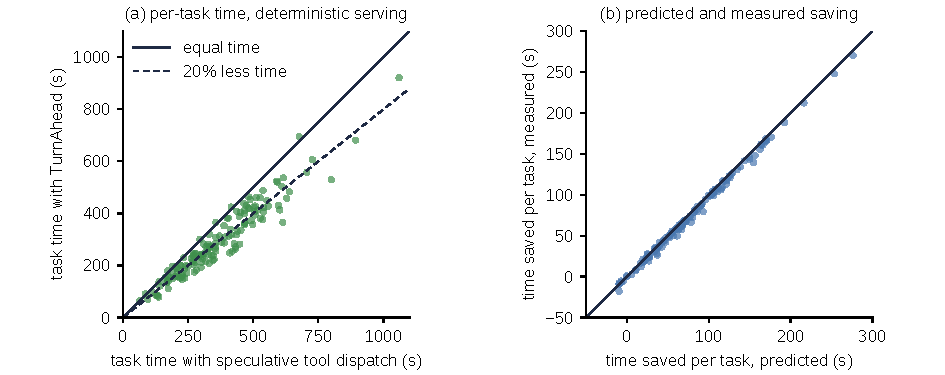
\includegraphics[width=0.92\textwidth]{figures/fig3_results.pdf}
\caption{Deterministic serving, one point per task. (a) Task time with \method against task time with speculative tool dispatch. (b) Time that \method saves over speculative tool dispatch: prediction of the cost model of \cref{sec:exp:analysis}, computed from the dispatch-only run, against the measurement.}
\label{fig:results}
\end{figure*}


\subsection{Trajectory Fidelity and Task Quality}
\label{sec:exp:fidelity}

\paragraph{Deterministic serving.}
On the \DetIdentClean{} tasks that complete, the generated tokens of all \DetIdentTurns{} turns are identical across the configurations, and so are the tool calls, the observations, and the environment after every turn.
The other \DetIdentFailed{} tasks reach the token limit in the same turn, after the same tokens, in every configuration.
The ablation variants also match. Comparing each task and configuration with its own \ToolLowFloor\,s run, all \ToolMidIdentical{} trajectories at \ToolMidFloor\,s and all \ToolHighIdentical{} at \ToolHighFloor\,s reproduce the generated tokens, calls, observations, and database states.
All three configurations match \DetMatchOurs\% of the gold actions on completed tasks.
The sandbox was exercised in these runs: successors changed the database before their check in \MotStateTotal{} windows, \MotStateDiscarded{} of which ended in a discard, and no trace of a discarded change appears in a committed environment.

\paragraph{Standard serving.}
Under standard serving the complete token sequence matches in \StdSameOursDisp{} of \StdSamePairsOursDisp{} successful TurnAhead--dispatch pairs.
The share of gold actions performed is \StdMatchNone\% without speculation, \StdMatchDisp\% with speculative tool dispatch, and \StdMatchOurs\% with \method; \method and speculative tool dispatch differ by \StdMatchDiffOursDisp{} points [\StdMatchDiffOursDispLo, \StdMatchDiffOursDispHi].
The token limit is reached in \StdFailNone, \StdFailDisp, and \StdFailOurs{} of \StdRunsOurs{} runs, respectively; here the two differ by \StdFailDiffOursDisp{} points [\StdFailDiffOursDispLo, \StdFailDiffOursDispHi].

\subsection{Ablation Study}
\label{sec:exp:ablation}

\begin{table}[t]
\centering
\small
\setlength{\tabcolsep}{4pt}
\begin{tabular}{lrl}
\toprule
Variant & Mean (s) & Saving (\%) \\
\midrule
Speculative tool dispatch & \AblMeanDisp & -- \\
\method & \AblMeanOurs & \AblSaveOurs{} [\AblSaveOursLo, \AblSaveOursHi] \\
\quad deferred tools & \AblMeanDefer & \AblSaveDefer{} [\AblSaveDeferLo, \AblSaveDeferHi] \\
\quad no successor probes & \AblMeanNoProbe & \AblSaveNoProbe{} [\AblSaveNoProbeLo, \AblSaveNoProbeHi] \\
\quad start after check & \AblMeanLate & \AblSaveLate{} [\AblSaveLateLo, \AblSaveLateHi] \\
\bottomrule
\end{tabular}
\caption{Variants of \method under deterministic serving (\AblTasks{} tasks). Savings are relative to speculative tool dispatch.}
\label{tab:ablation}
\end{table}

\Cref{tab:ablation} isolates the contributions of early launch, sandboxed tools, and successor probes at the \ToolLowFloor\,s floor.

\paragraph{Start after the check.}
This variant builds the same successor input but runs the check first and starts the successor only if it passes, so parent and successor never overlap.
Its saving vanishes (\AblSaveLate\%).
The gain of \method thus comes entirely from running the next turn inside the parent's slack, and the bookkeeping of a window costs almost nothing.

\paragraph{Deferred tool execution.}
This is the mode of \cref{sec:method:sandbox} that holds the successor's tool calls until the commit decision.
It is \AblSlowerDefer\% slower than the full method [\AblSlowerDeferLo, \AblSlowerDeferHi].

\paragraph{No probes in the successor.}
Without speculative tool dispatch inside the successor, the successor's own tool call is no longer overlapped with its reasoning.
This variant is \AblSlowerNoProbe\% slower than the full method [\AblSlowerNoProbeLo, \AblSlowerNoProbeHi].

Longer tool calls increase the value of probing inside the successor. Removing these probes slows \method by \ToolMidNoProbe\% at \ToolMidFloor\,s and \ToolHighNoProbe\% at \ToolHighFloor\,s. Deferring successor tools until commit has a smaller cost at the same floors (\ToolMidDefer\% and \ToolHighDefer\%). Deferral delays a tool only when the successor reaches it before the parent commits.

\subsection{When Does \method Help?}
\label{sec:exp:analysis}

\paragraph{Windows.}
Under deterministic serving, a successor is started in \WinDetStarted{} of \WinDetWindows{} windows and committed in \WinDetCommitted{} of them (\WinDetCommitPct\%).
Of the \WinDetDiscarded{} discarded successors, \WinDetRejReply{} belong to parents that replied to the user instead of calling a tool and \WinDetRejCall{} to parents that emitted a different call.
The remaining \WinDetRejInput{} belong to parents whose call matched but whose output added something to the history, so that only the input check rejected them.
Under standard serving the commit rate is \WinStdCommitPct\% (\WinStdCommitted{} of \WinStdStarted{} successors).

\paragraph{The cost of a second request.}
While parent and successor overlap, they share the server.
We measure the cost of sharing separately, by decoding the same prompts alone and two at a time (\cref{app:impl}).
Each of two concurrent requests is slowed by a factor of $s=\ConDetTwo$ under deterministic serving and $s=\ConStdTwo$ under standard serving.
According to \cref{sec:method:overview}, a committed window then saves $(2-s)\,\Delta T_t$, and a discarded one costs $(s-1)$ times its overlap.
We apply this model to the runs of speculative tool dispatch, which contain no successors, and predict from them what \method should save (\cref{app:results}).
The prediction is \CostDetPred\% under deterministic serving, where we measure \CostDetMeasured\%, and \CostStdPred\% under standard serving, where we measure \CostStdMeasured\%.
Per task, the predicted and the measured savings under deterministic serving correlate with $r=\CostDetCorr$ (\cref{fig:results}b).

The model also accounts for the gap between the two serving modes.
Without contention ($s=1$) it gives \CostDetIdeal\% and \CostStdIdeal\%.
This part of the gap lies in the workload: turns are shorter under standard serving, so the fixed tool latency takes a larger part of them (the observation is ready after \MotStdReadyPosPct\% of a turn instead of \MotReadyPosPct\%), and fewer turns dispatch a correct call (\MotStdAnchorPct\% instead of \MotAnchorPct\%).
Contention then removes \CostDetContention{} points under deterministic serving and \CostStdContention{} under standard serving.
The second request adds a similar time per token in both modes (\ConDetExtraMs\,ms and \ConStdExtraMs\,ms), which is a larger fraction when a single request decodes faster.
Committed successors account for \WinDetOverlapCommitPct\% of observed overlap time under deterministic serving and \WinStdOverlapCommitPct\% under standard serving. Both exceed the respective break-even shares of \CostDetBreakeven\% and \CostStdBreakeven\%.

\paragraph{Overhead.}
\method generates more tokens than it commits.
Counting probes and discarded successors, speculative tool dispatch generates \OvhDetGenDisp{} tokens per committed token and \method generates \OvhDetGenOurs.
Discarded successors alone amount to \OvhDetLostPctOurs\% of the committed tokens (\OvhStdLostPctOurs\% under standard serving).
On a dedicated server this work uses capacity that the serial loop leaves idle, and its effect on latency is already part of the measured times.

\paragraph{Can discarded work be reused?}
A discarded successor could serve as a token-level draft for the turn that replaces it.
The replaced turns hold \ReuseDetReplacedPct\% of the committed tokens.
Runs of at least eight tokens that a replaced turn shares with its discarded successor cover \ReuseDetSharedPct\% of its tokens, which is \ReuseDetSharedAllPct\% of all committed tokens (\ReuseStdSharedAllPct\% under standard serving).
A successor is usually discarded because the parent decided otherwise, and it then reasons about an observation that the real turn never sees.

\paragraph{Tool latency.}
Longer tool calls shift the gain toward early dispatch (\cref{fig:tool-latency}). Raising the floor from \ToolLowFloor{} to \ToolHighFloor\,s increases the saving of dispatch over serial execution from \ToolLowDispatch\% to \ToolHighDispatch\%.
The observation also arrives later, leaving less parent reasoning in which to run a successor. The additional saving over dispatch falls from \ToolLowIncrement\% to \ToolMidIncrement\% and then \ToolHighIncrement\%.
Together, dispatch and early successor execution save \ToolLowTotal\%, \ToolMidTotal\%, and \ToolHighTotal\% over serial execution at the three floors.

\begin{figure}[t]
\centering
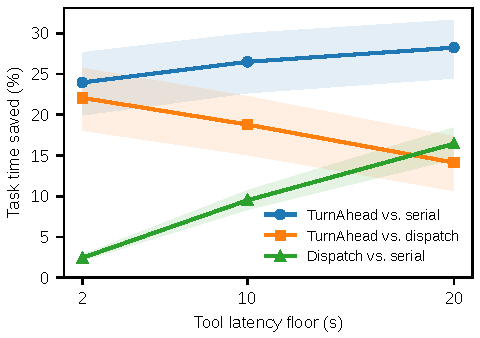
\includegraphics[width=\columnwidth]{figures/fig4_tool_latency.pdf}
\caption{Task time saved as tool latency increases on the same \AblTasks{} tasks. Shading gives task-bootstrap 95\% intervals.}
\label{fig:tool-latency}
\end{figure}

% !TEX root = ../main.tex
\section{Conclusion}
\label{sec:conclusion}

\method runs the next turn of a reasoning agent as soon as a speculative tool call returns. Its commit check lets the agent use that work when the next input and environment match. On Qwen3-32B, this reduces task time over tool dispatch by \DetSaveOursDisp\% under deterministic serving and \StdSaveOursDisp\% under standard serving. The latency sweep shows how the two forms of overlap complement each other: faster tools leave more reasoning time for the successor, while slower tools reward earlier dispatch.

% !TEX root = ../main.tex
\section*{Limitations}

\paragraph{History policy.}
\method relies on a history that keeps only the final output of earlier turns.
If a harness keeps their reasoning, the input of a successor can never match the real one, every successor is discarded, and \method should be switched off.

\paragraph{Depth.}
Windows are disjoint and one turn deep, so at most every second turn starts early.
Deeper speculation would add concurrent requests and discarded work, and we do not evaluate it.

\paragraph{Sandboxing.}
Copy-based sandboxing requires an environment whose state can be copied.
Tools with external effects need the deferred mode, which we evaluate only on \taubench, where it is not required.

\paragraph{Determinism.}
The guarantee of identical trajectories requires deterministic decoding.
We verify it with batch-invariant kernels within one server instance and with greedy decoding.
With standard kernels, outputs depend on batching for every method that issues concurrent requests, and we can only compare aggregates.

\paragraph{Compute and sharing.}
\method generates \OvhDetGenOurs{} tokens per committed token, and its gain shrinks as a second concurrent request becomes more expensive.
All experiments use a dedicated server and one agent at a time.
On a shared server, successors would compete with the requests of other users, which we do not evaluate.

\paragraph{Evaluation.}
The tasks give the user's request in a single message and are scored by their gold actions, not by the interactive success rate of the benchmark, and tool latency is a fixed floor.


\bibliography{references}

\appendix
% !TEX root = ../main.tex
\section{Implementation Details}
\label{app:impl}

\paragraph{Serving and decoding.}
All methods use the same vLLM~0.29 server~\citep{kwon2023vllm} and the same request settings.
Qwen3-32B is served in 16-bit precision with tensor parallelism over four RTX~3090 GPUs (24\,GB each), with prompt-lookup speculative decoding of up to 20 tokens.
Decoding is greedy with a fixed seed, at most 8{,}192 new tokens per turn, and a context window of 40{,}960 tokens.
Deterministic serving switches the server to batch-invariant mode, in which the output of a request does not depend on the requests decoded with it.
All configurations of an experiment use one server instance, and we do not rely on outputs being reproducible across server restarts.
A request that runs alone decodes at \SpdDetMsSolo\,ms per token under deterministic serving and at \SpdStdMsSolo\,ms under standard serving.

\paragraph{Cost of concurrent requests.}
We decode the first turn of four retail tasks alone and then two, three, and four of them at the same time, 320 tokens each, three times over.
For every request we compare the time it needs for the same token positions, alone and while all requests are active.
The median slowdown for two, three, and four concurrent requests is \ConDetTwo, \ConDetThree, and \ConDetFour{} under deterministic serving and \ConStdTwo, \ConStdThree, and \ConStdFour{} under standard serving.
The main runs agree with this: a parent whose successor runs during part of its turn decodes \SpdDetBusyRatio$\times$ and \SpdStdBusyRatio$\times$ slower than a turn without speculation in the two modes.

\paragraph{Speculative tool dispatch.}
The first probe is issued when the first token of a turn arrives, and further probes follow about every 50 generated tokens, at sentence boundaries, up to five per turn.
A probe may generate up to 160 tokens.
A call is dispatched when the minimum token probability over positions two through sixteen of the probe continuation is at least 0.9, and at most one call is dispatched per turn.
These settings are the same for the baseline, for the parent, and for the successor.

\paragraph{Tools and environment copies.}
The tools of \taubench run against the benchmark's local database and return within milliseconds.
All methods use the same tool latency floor within each comparison (\ToolLowFloor, \ToolMidFloor, or \ToolHighFloor\,s).
An environment copy is a deep copy of the benchmark environment.
Creating it adds a median of \MotCopyMedian\,s between the dispatch decision and the start of the tool.
The fingerprint of an environment is the pair of hashes of its agent-side and user-side databases.

\paragraph{The check.}
Observations are compared by SHA-256.
The configuration compared by condition~(v) consists of the model, the endpoint, the seed, the token budget, the context window, the thinking flag, the stop strings, the temperature, and the presence penalty.

\paragraph{Successor.}
The successor uses the settings of a regular turn with one exception.
It does not reuse probe tokens as drafts, because our server keeps a single draft state that is shared by all requests.
The parent keeps this optimization.
The drafts that the successors forgo would save at most \MotDraftForgonePct\% of the time.

\paragraph{History.}
For all methods, the assistant message stored in the history is the output of the turn with its reasoning block removed.

% !TEX root = ../main.tex
\section{Why Committed Trajectories Match Serial Execution}
\label{app:consistency}

This appendix spells out the argument behind the guarantee of \cref{sec:method:commit} and derives the savings stated in \cref{sec:method:overview}.

\paragraph{Conditions.}
The argument rests on four conditions.
First, decoding is deterministic: for a fixed input and configuration, the output that enters the history does not depend on which other requests are being decoded.
Second, the environment is deterministic: the result of a tool and the new environment depend only on the current environment and the call, and equal fingerprints mean equal environments.
Third, speculative executions touch only copies, and a copy becomes the environment only through adoption.
Fourth, nothing changes the committed history or environment between the final check and adoption.

\paragraph{Argument.}
We compare \method with serial execution window by window and assume that both start a window with the same history and environment.
The parent receives the same input in both executions and therefore produces the same output.
Its call is committed either by adopting the copy on which the dispatched call ran, which requires the two calls to be equal, or by executing the call directly.
In both cases the observation and the new environment are those of serial execution.
If the successor passes the check, it has the input and configuration of the serial turn $t{+}1$ and started from the same environment.
It therefore produces the same output, the same tool result, and the same new environment, and adoption makes exactly these the committed ones.
If the successor is discarded, it leaves nothing behind, and turn $t{+}1$ runs as in serial execution.
Either way, both executions end the window with the same history and environment, so the next window starts from the same point.

\paragraph{The parent's entry in the history.}
When a successor is committed, the history holds the parent's entry in the form the successor used, built from the dispatched call, instead of the parent's raw output.
The input check shows that both forms render to the same tokens.
Because the chat template renders each message from its own content and role, they also render identically in every later input.

\paragraph{If reasoning were kept in the history.}
The guarantee does not depend on the history policy of \cref{sec:motivation:input}.
If a harness kept reasoning in the history, the successor's input would never match and every successor would be discarded.
\method would remain lossless but would bring no gain, and it should be disabled.

\paragraph{Sampling.}
With stochastic decoding, the argument holds if the output of each turn is a deterministic function of its input, its configuration, and its random seed, and if the successor uses the seed of the turn it stands for.
A discarded successor must not be resampled or selected by its outcome, because this would change the distribution of committed outputs.
\method never does so.
All our experiments use greedy decoding.

\paragraph{Derivation of \cref{eq:saving}.}
Measure time from the start of the parent, and assume that the anchor is correct and ready before the parent ends, $\tau_t\le R_t$.
With speculative tool dispatch alone, the parent ends at $R_t$ and turn $t{+}1$ then takes $B_{t+1}$, for a total of $R_t+B_{t+1}$.
With \method, the successor starts at $\tau_t$ and ends at $\tau_t+B_{t+1}$, and the window ends when both turns are done, at $\max(R_t,\tau_t+B_{t+1})$.
The difference is $\min(B_{t+1},R_t-\tau_t)$.
A window cannot end before its longer turn, and without \method it takes at most twice as long as that turn, so the speedup of a window is at most $2\times$.
If the anchor is not ready before the parent ends, no successor is started and nothing is saved.

\paragraph{Contention.}
Now let each of two concurrent requests progress at rate $1/s$, and write $m=\min(B_{t+1},\sigma_t)$ with $\sigma_t$ and $B_{t+1}$ measured without contention.
If $B_{t+1}\ge\sigma_t$, the parent needs $s\sigma_t$ instead of $\sigma_t$ to finish after the anchor, and the successor completes work worth $\sigma_t$ in that time.
The window then ends $s\sigma_t+B_{t+1}-\sigma_t$ after the anchor instead of $\sigma_t+B_{t+1}$, which saves $(2-s)\,\sigma_t$.
If $B_{t+1}<\sigma_t$, the successor needs $sB_{t+1}$, the parent advances by $B_{t+1}$ in that time and then continues alone, and the window ends $\sigma_t+(s-1)B_{t+1}$ after the anchor, which saves $(2-s)\,B_{t+1}$.
In both cases a committed window saves $(2-s)\,m$.
A discarded successor contributes nothing and slows the parent for as long as both run.
If it would have run alone for $m'$ of the slack, the parent ends $(s-1)\,m'$ later.
With a commit rate $p$ and overlaps of similar length in both cases, a started window saves $p\,(2-s)\,m-(1-p)(s-1)\,m=(p-(s-1))\,m$ on average.

% !TEX root = ../main.tex
\section{Additional Results}
\label{app:results}

\begin{table*}[t]
\centering
\small
\setlength{\tabcolsep}{4pt}
% Generated by scripts/results_stats.py. Do not edit by hand.
\begin{tabular}{lrrrlrrrl}
\toprule
 & \multicolumn{4}{c}{Deterministic serving} & \multicolumn{4}{c}{Standard serving} \\
\cmidrule(lr){2-5}\cmidrule(lr){6-9}
Tasks & Runs & Dispatch (s) & \method (s) & Saving (\%) & Runs & Dispatch (s) & \method (s) & Saving (\%) \\
\midrule
All tasks & 148 & 366.7 & 293.7 & 19.9\,[18.1,\,21.6] & 270 & 134.8 & 117.7 & 12.7\,[7.2,\,17.9] \\
Airline & 40 & 354.1 & 290.3 & 18.0\,[14.2,\,21.9] & 77 & 149.5 & 126.0 & 15.7\,[6.0,\,24.6] \\
Retail & 108 & 371.4 & 295.0 & 20.6\,[18.7,\,22.5] & 193 & 129.0 & 114.4 & 11.3\,[4.4,\,17.8] \\
\bottomrule
\end{tabular}

\caption{Mean task time with speculative tool dispatch and with \method by domain, with the saving and its 95\% bootstrap interval.}
\label{tab:breakdown}
\end{table*}

\paragraph{Domains.}
\Cref{tab:breakdown} splits the comparison of \method with speculative tool dispatch by domain.

\paragraph{Motivation statistics under standard serving.}
The analysis of \cref{sec:motivation} gives the same picture under standard serving.
A correct call is dispatched in \MotStdAnchorPct\% of the tool-calling turns, and its observation is ready after a median of \MotStdReadyPosPct\% of the turn's generation time.
The median slack is \MotStdSlackMedian\,s (\MotStdSlackSharePct\% of the turn), and the median ratio of slack to next-turn duration is \MotStdSlackOverNext.
The whole next turn fits into the slack in \MotStdNextFitsPct\% of the pairs and at least half of it in \MotStdNextHalfPct\%.
The next input built from the dispatched call is identical to the real one in \MotStdInputSamePct\% of the cases.

\paragraph{Predicting the saving.}
For \cref{sec:exp:analysis} we form the windows of \method in the runs of speculative tool dispatch.
A window has a successor if its parent dispatched a call whose observation arrived before the parent's reasoning ended.
It commits if the dispatched call equals the parent's call and the input built from it equals the real next input, which is the test of \cref{sec:motivation:input}.
Its overlap is the smaller of the slack and the duration of the next turn if it commits, and the smaller of the slack and the median turn duration otherwise.
The predicted saving of a task is $(2-s)$ times the overlap of its committing windows minus $(s-1)$ times the overlap of the others, with $s$ taken from the measurement of \cref{app:impl}.
Under standard serving, where each task has its own trajectory in every configuration, the prediction is meaningful only in aggregate.

\paragraph{Repeated runs under standard serving.}
Two runs of the same task yield the same tokens in \StdRepeatSameNone{} of \StdRepeatPairsNone{} cases without speculation, in \StdRepeatSameDisp{} of \StdRepeatPairsDisp{} with speculative tool dispatch, and in \StdRepeatSameOurs{} of \StdRepeatPairsOurs{} with \method.
The more of a turn overlaps with other requests, the less reproducible its output is under standard kernels.


\end{document}
